\documentclass[a4paper, 12pt, english]{article}

% \usepackage[portuges]{babel}
\usepackage[utf8]{inputenc}
\usepackage{amsmath,amssymb}
\usepackage{graphicx}
\usepackage{subfig}
\usepackage[colorinlistoftodos]{todonotes}

\usepackage{indentfirst}
\usepackage{verbatim}
\usepackage{textcomp}
\usepackage{gensymb}

\usepackage{relsize}

\usepackage{lipsum}% http://ctan.org/pkg/lipsum
\usepackage{xcolor}% http://ctan.org/pkg/xcolor
\usepackage{xparse}% http://ctan.org/pkg/xparse
\NewDocumentCommand{\myrule}{O{1pt} O{2pt} O{black}}{%
  \par\nobreak % don't break a page here
  \kern\the\prevdepth % don't take into account the depth of the preceding line
  \kern#2 % space before the rule
  {\color{#3}\hrule height #1 width\hsize} % the rule
  \kern#2 % space after the rule
  \nointerlineskip % no additional space after the rule
}
\usepackage[section]{placeins}

\usepackage{booktabs}
\usepackage{colortbl}%
   \newcommand{\myrowcolour}{\rowcolor[gray]{0.925}}
   
\usepackage[obeyspaces]{url}
\usepackage{etoolbox}
\usepackage[colorlinks,citecolor=black,urlcolor=blue,bookmarks=false,hypertexnames=true]{hyperref} 

\usepackage{geometry}
\geometry{
	paper=a4paper, % Change to letterpaper for US letter
	inner=3cm, % Inner margin
	outer=3cm, % Outer margin
	bindingoffset=.5cm, % Binding offset
	top=2cm, % Top margin
	bottom=2cm, % Bottom margin
	%showframe, % Uncomment to show how the type block is set on the page
}

\usepackage{float}

\usepackage{amsmath,amsfonts}


\usepackage{multicol,caption}
\newenvironment{Figure}
  {\par\medskip\noindent\minipage{\linewidth}}
  {\endminipage\par\medskip}
\usepackage{array}

\newcommand{\highlight}[1]{\textcolor{blue}{\texttt{#1}}}

\graphicspath{{images/}}

\newlength{\simheight}
\settoheight{\simheight}{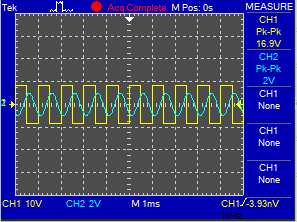
\includegraphics{images/Inverting-Schmitt-Trigger-Sim.png}}

\newlength{\vrefheight}
\settoheight{\vrefheight}{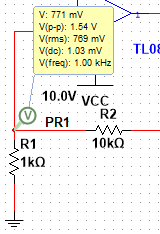
\includegraphics{images/Inverting-Schmitt-Trigger-Vref-Circuit.png}}

%*******************************************************************************%
%************************************START**************************************%
%*******************************************************************************%
\begin{document}

%************************************TITLE PAGE**************************************%
\begin{titlepage}
\begin{center}
\textbf{\LARGE Alexandria University}\\[0.5cm] 
\textbf{\large FACULTY OF ENGINEERING}\\[0.2cm]
\vspace{20pt}

\includegraphics{logo.png}\\[1cm]
\par
\vspace{20pt}
\textbf{\Large EEC332 Analog Integrated Circuits}\\
\vspace{15pt}
\myrule[1pt][7pt]
\textbf{\LARGE  Experiment 3}\\
\vspace{15pt}
\textbf{\large Study the characteristics of regenerative feedback
system with extension to design an astable and
monostable multivibrator}\\
\myrule[1pt][7pt]
\vspace{25pt}
\textbf{\large \hspace{50pt}Student Name \hspace{60pt} Student ID}\\
Ahmed Osama Mohamed Afifi \hspace{60pt} 20010038 \\
Ziad Mohamed Mohamed Abdalla \hspace{40pt} 20010643 \\

\vspace{45pt}
%\textbf {\large Lecturer in charge:}\\[0.2cm]
%\Large {Ir. Chan Cheong Loong}\\[0.1cm]
\end{center}

\par
\vfill
\begin{center}
\textbf{Submission Date : 09/05/2024}\\
\end{center}

\end{titlepage}

%************************************TABLE OF CONTENTS**************************************%

%  %Sumário
%  \newpage
%  \tableofcontents
%  \thispagestyle{empty}
%  %End Sumário

%********************************%
%***********SECTION 1************%
%********************************%
\newpage
\section{Introduction}
In this laboratory, we delve into the realm of inverting regenerative comparators and astable multivibrators, exploring their roles as essential elements in signal processing, waveform generation, and electronic switching. By harnessing the amplification and feedback capabilities of op-amps, these circuits transcend mere signal amplification, offering precision, stability, and versatility in a myriad of applications.
\newline

%********************************%
%***********SECTION 2************%
%********************************%
\section{Inverting Schmitt Trigger}
\subsection{Schematic}
\begin{figure}[H]
 \centering
 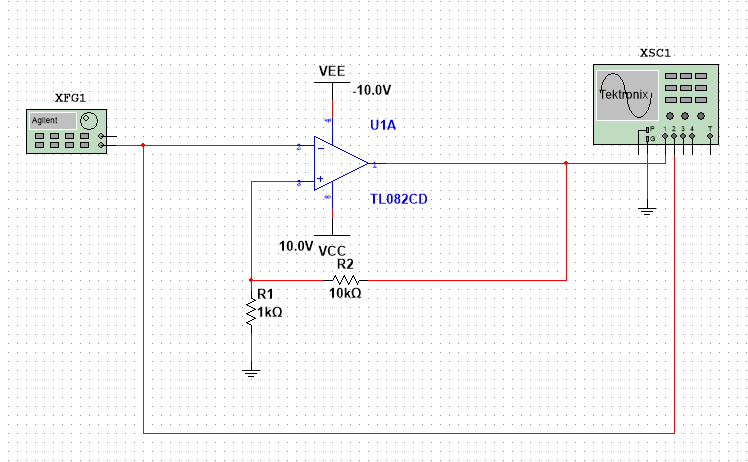
\includegraphics[width=\linewidth]{images/Inverting-Schmitt-Trigger.png}
 \caption{Inverting Schmitt Trigger}
 \label{fig:Inverting Schmitt Trigger}
\end{figure}


\subsection{Results}

\subsubsection{Lab results}
\begin{figure}[H]
    \centering
    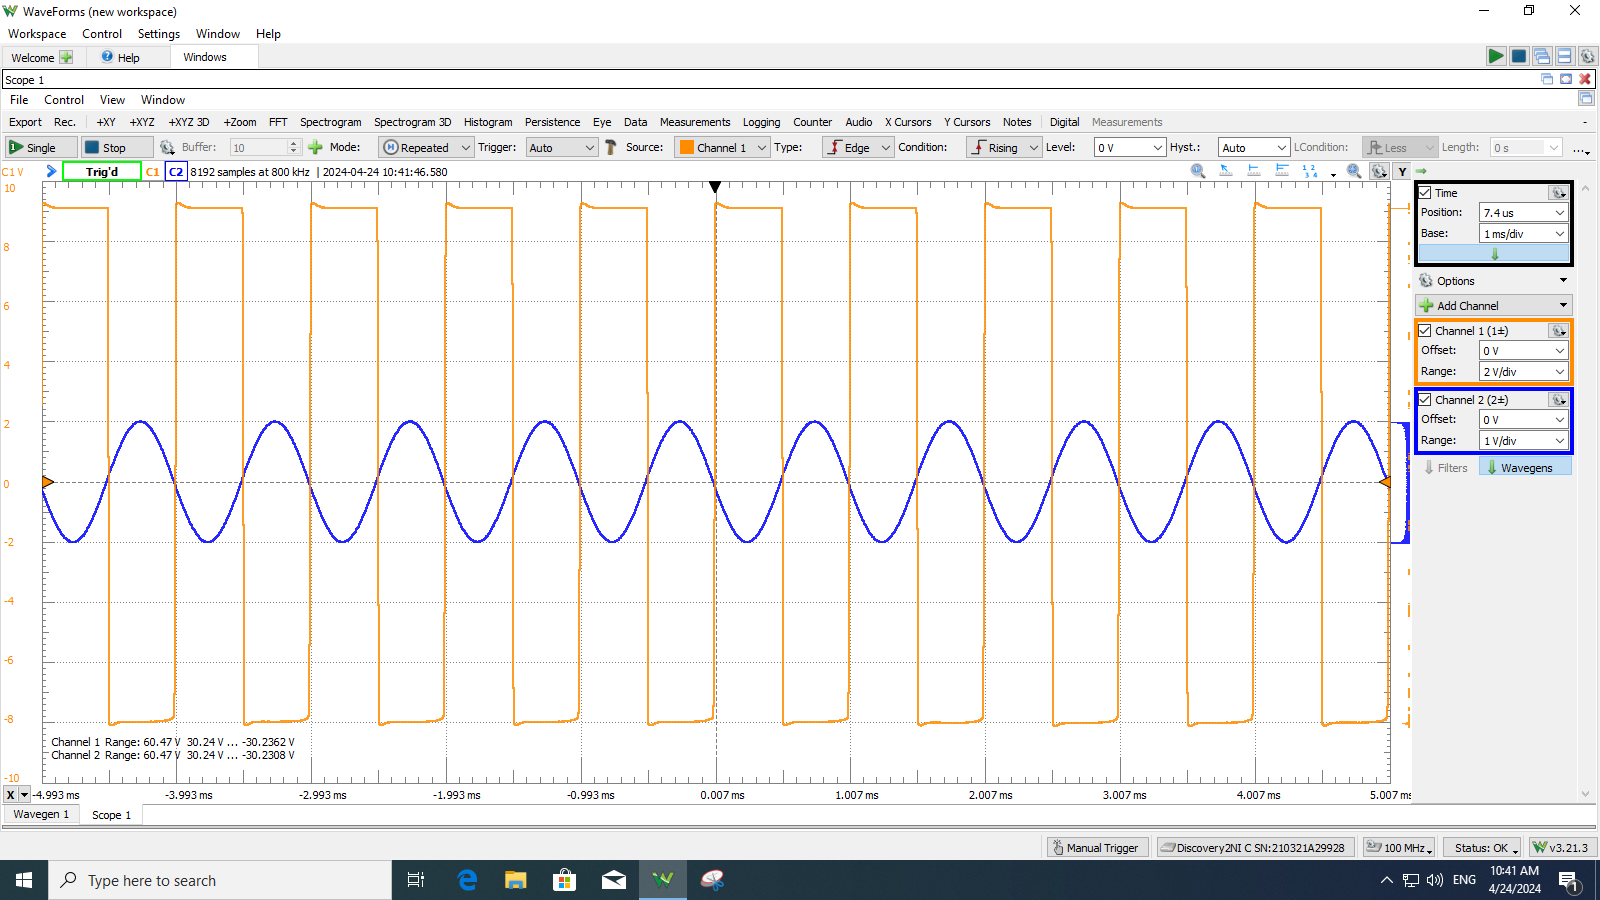
\includegraphics[width=\linewidth]{images/Inverting-Schmitt-Trigger-Lab.png}
    \caption{Lab result for inverting schmitt-trigger with sinusoidal wave input}
    \label{fig:Lab result for inverting schmitt-trigger with sinusoidal wave input}
\end{figure}


\subsubsection{Simulation results}
\begin{figure}[H]
    \centering
    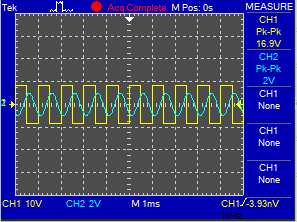
\includegraphics[width=\linewidth, height=\simheight]{images/Inverting-Schmitt-Trigger-Sim.png}
    \caption{Simulation result for inverting schmitt-trigger with sinusoidal wave input}
    \label{fig:Simulation result for inverting schmitt-trigger with sinusoidal wave input}
\end{figure}

% \begin{multicols}{2}
% \begin{tabular}{>{\raggedright}p{\linewidth} >{\raggedleft}p{\linewidth}}
% \begin{Figure}
%  \centering
%  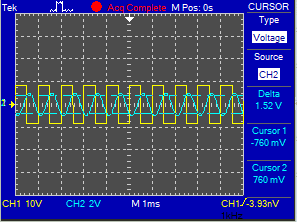
\includegraphics[width=\linewidth, height=0.5\vrefheight]{images/Inverting-Schmitt-Trigger-Vref-Cursor.png}
%  \captionof{figure}{$V_{ref}$ from waveform}
% \end{Figure} & \begin{Figure}
%  \centering
%  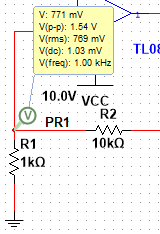
\includegraphics[width=\linewidth, height=0.5\vrefheight]{images/Inverting-Schmitt-Trigger-Vref-Circuit.png}
%  \captionof{figure}{$V_{ref}$ from circuit}
% \end{Figure}
% \end{tabular}
% \end{multicols}

\begin{figure}[H]
    \centering
    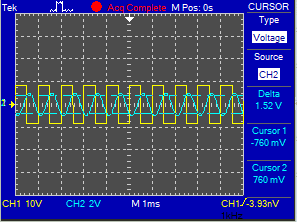
\includegraphics[width=\linewidth, height=\simheight]{images/Inverting-Schmitt-Trigger-Vref-Cursor.png}
    \caption{$V_{ref}$ from waveform for inverting schmitt trigger}
    \label{fig:$V_{ref}$ from waveform for inverting schmitt trigger}
\end{figure}

\subsection{Comments}
One of the primary features of a Schmitt trigger is its hysteresis loop, which results in two distinct switching thresholds. As the input signal crosses these thresholds, the output transitions between high and low states. The width of the hysteresis loop is determined by the feedback resistor and the input resistors' ratio. 
\[ \|V_{ref}| = \frac{R_{1}}{R_{1} + R_{2}}  \times V_{ss}\]
Where, \begin{itemize}
    \item $|V_{ref}|$: is the threshold voltage.
    \item $V_{ss}$: is the supply voltage.
\end{itemize}
From the electrical characteristics of the used OP-AMP TL082, the Output swing headroom to negative supply is $+1.5 V$, and to positive supply is $-1.5 V$. Hence in our case, the supply voltage is $\pm{10V}$. Thus, $|V_{ss}|=8.5$ and \(|V_{ref}|=\frac{1k}{1k+10k}\times8.5=772mV\). \\
From figure \ref{fig:$V_{ref}$ from waveform for inverting schmitt trigger}, $|V_{ref}|=760mV$ which is near the theoretical value.

\newpage
%********************************%
%***********SECTION 3************%
%********************************%
\section{Non-Inverting Schmitt Trigger}
\subsection{Schematic}
\begin{figure}[H]
 \centering
 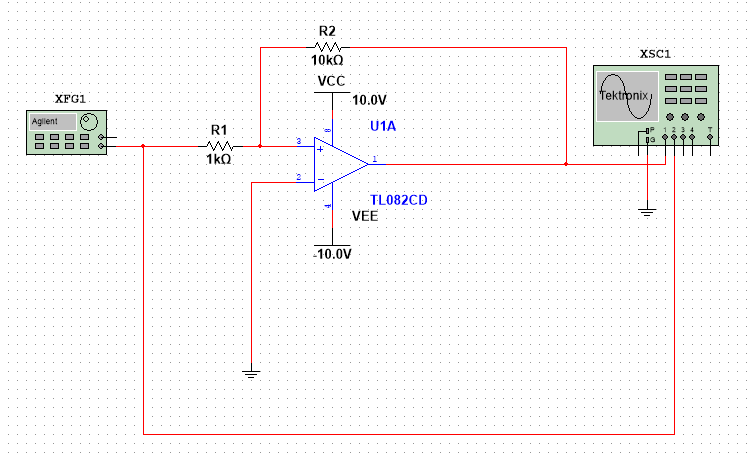
\includegraphics[width=\linewidth]{images/Non-Inverting-Schmitt-Trigger.png}
 \caption{Non-inverting Schmitt Trigger}
 \label{fig:Non-inverting Schmitt Trigger}
\end{figure}


\subsection{Results}

\subsubsection{Lab results}
\begin{figure}[H]
    \centering
    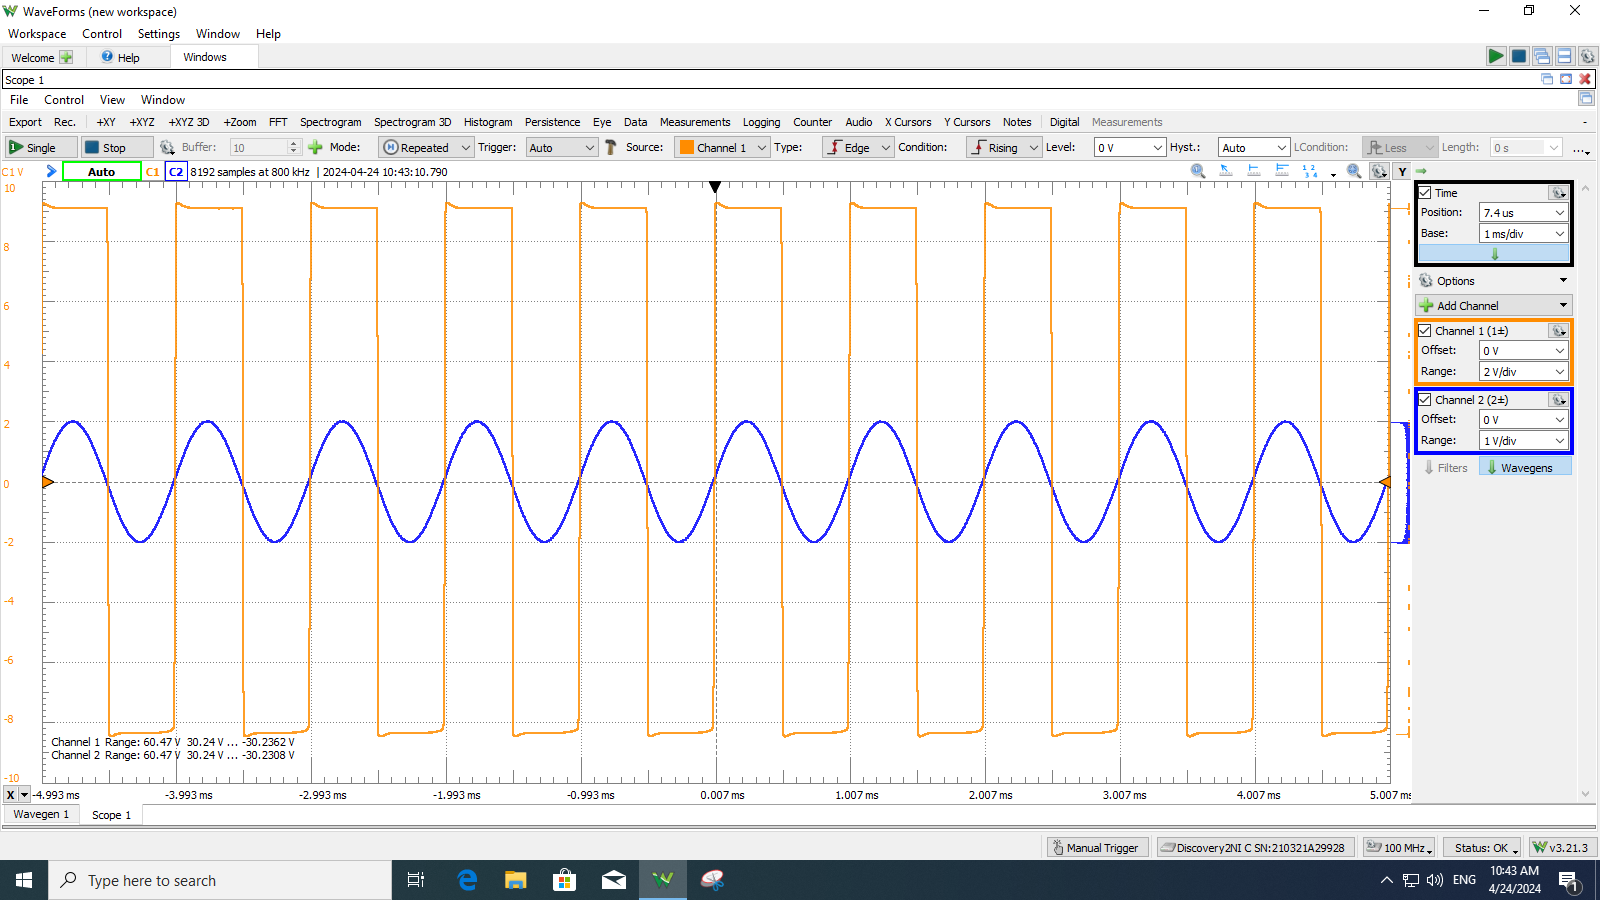
\includegraphics[width=\linewidth]{images/Non-Inverting-Schmitt-Trigger-Lab.png}
    \caption{Lab result for non-inverting schmitt-trigger with sinusoidal wave input}
    \label{fig:Lab result for non-inverting schmitt-trigger with sinusoidal wave input}
\end{figure}


\subsubsection{Simulation results}
\begin{figure}[H]
    \centering
    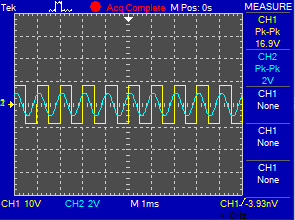
\includegraphics[width=\linewidth, height=\simheight]{images/Non-Inverting-Schmitt-Trigger-Sim.png}
    \caption{Simulation result for non-inverting schmitt-trigger with sinusoidal wave input}
    \label{fig:Simulation result for non-inverting schmitt-trigger with sinusoidal wave input}
\end{figure}

\begin{figure}[H]
    \centering
    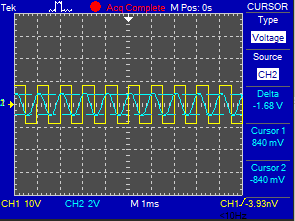
\includegraphics[width=\linewidth, height=\simheight]{images/Non-Inverting-Schmitt-Trigger-Vref-Cursor.png}
    \caption{$V_{ref}$ from waveform for non-inverting schmitt trigger}
    \label{fig:$V_{ref}$ from waveform for non-inverting schmitt trigger}
\end{figure}

\subsection{Comments}
Like the inverting Schmitt trigger, the non-inverting configuration also exhibits hysteresis behavior, resulting in two distinct threshold levels for switching the output between high and low states. These threshold levels are determined by the resistor values in the feedback network and the input resistors' ratio.
\[ |V_{ref}| = \frac{R_{1}}{R_{2}}  \times V_{ss}\]
Thus, \(|V_{ref}|=\frac{1k}{10k}\times8.5=850mV\). \\
From figure \ref{fig:$V_{ref}$ from waveform for non-inverting schmitt trigger}, $|V_{ref}|=850mV$ which is near the theoretical value.

\newpage

%********************************%
%***********SECTION 4************%
%********************************%
\section{Square Wave Generator}
\subsection{Schematic}
\begin{figure}[H]
 \centering
 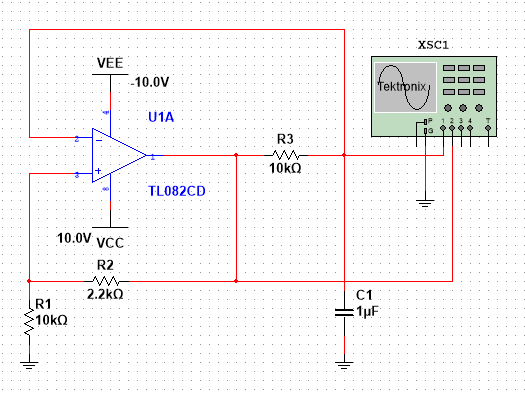
\includegraphics[width=\linewidth]{images/Square-Wave-Generator.png}
 \caption{Astable Multivibrator as Square Wave Generator}
 \label{fig:Astable Multivibrator as Square Wave Generator}
\end{figure}


\subsection{Results}

\subsubsection{Lab results}
\begin{figure}[H]
    \centering
    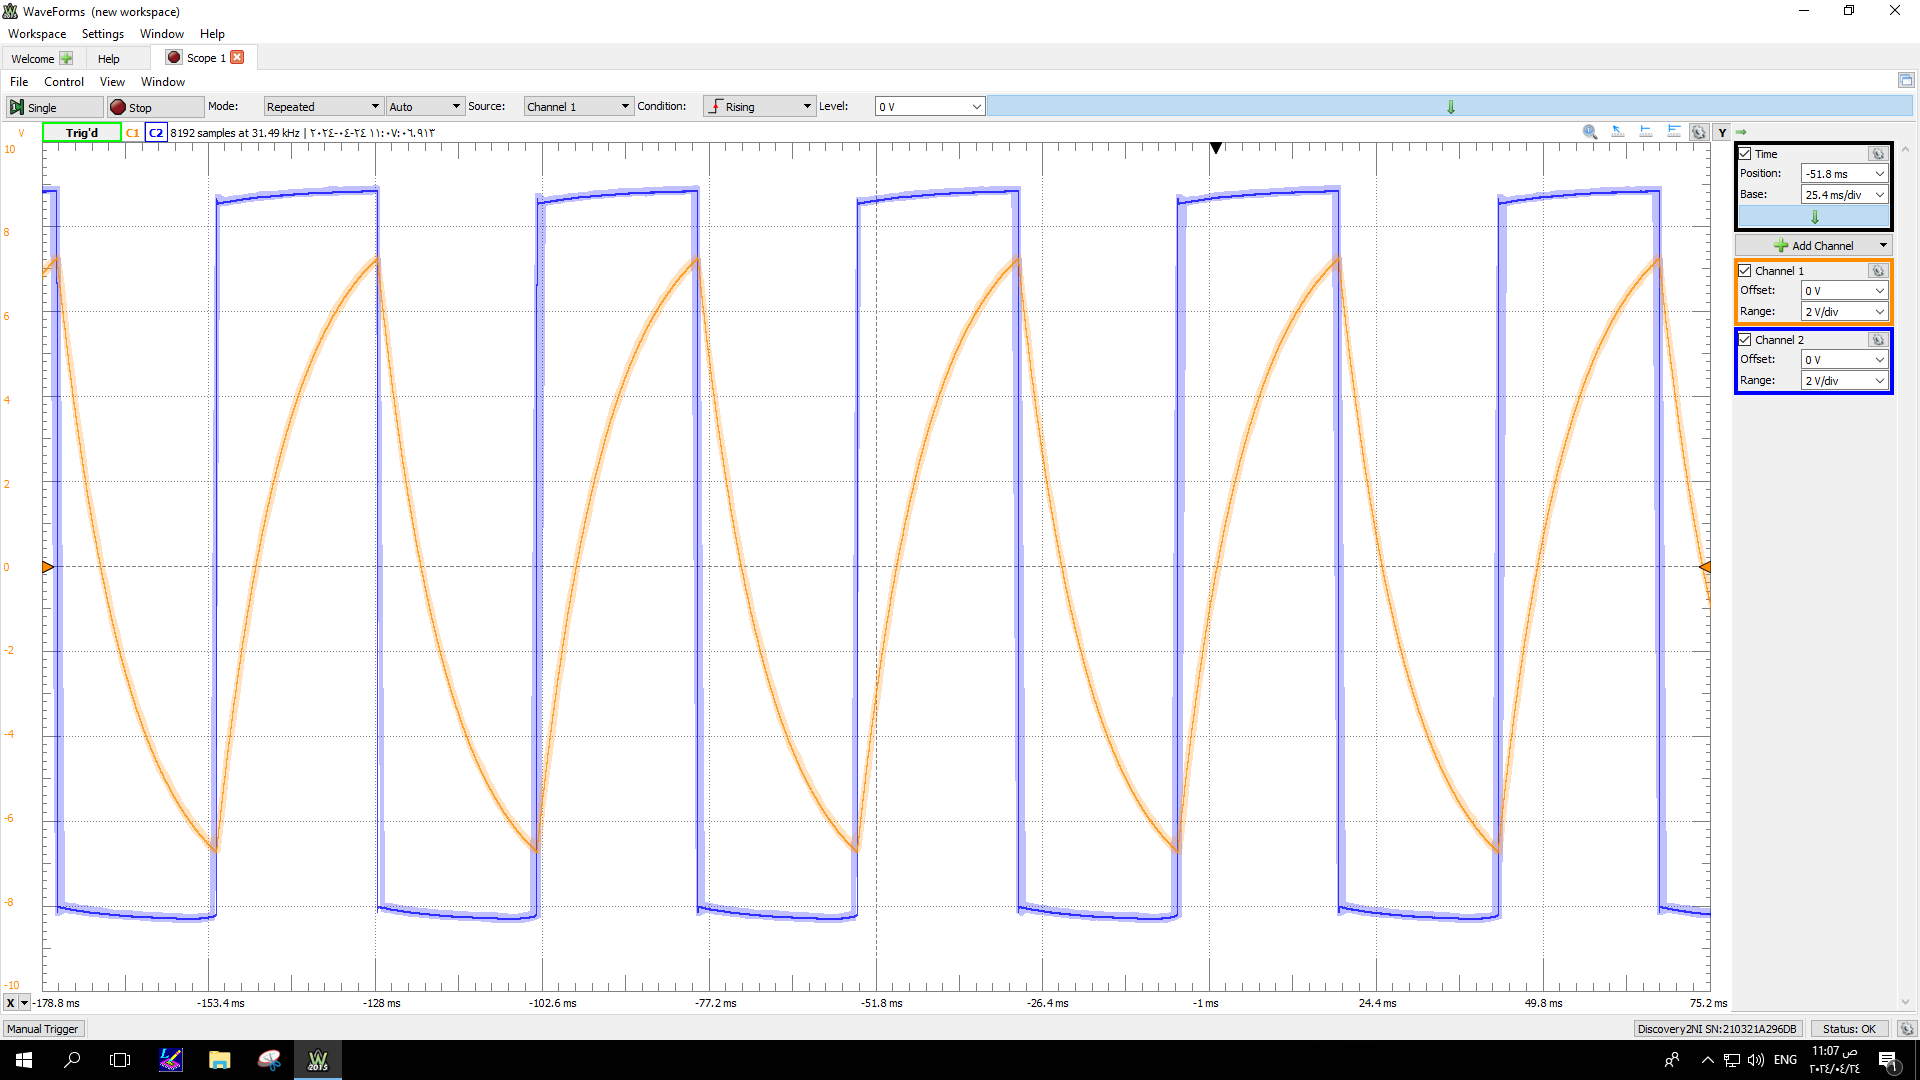
\includegraphics[width=\linewidth]{images/Square-Wave-Generator-Lab.png}
    \caption{Lab result for astable multivibrator as square wave generator}
    \label{fig:Lab result for astable multivibrator as square wave generator}
\end{figure}


\subsubsection{Simulation results}
\begin{figure}[H]
    \centering
    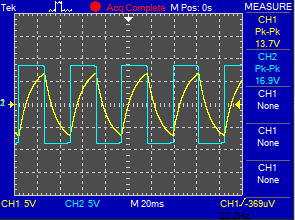
\includegraphics[width=\linewidth, height=\simheight]{images/Square-Wave-Generator-Sim.png}
    \caption{Simulation result for astable multivibrator as square wave generator}
    \label{fig:Simulation result for astable multivibrator as square wave generator}
\end{figure}

\begin{figure}[H]
    \centering
    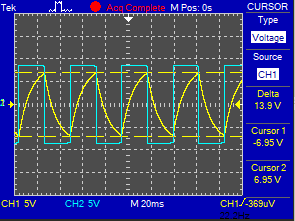
\includegraphics[width=\linewidth, height=\simheight]{images/Square-Wave-Generator-Vref-Cursor.png}
    \caption{$V_{ref}$ from waveform for astable multivibrator as square wave generator}
    \label{fig:$V_{ref}$ from waveform for astable multivibrator as square wave generator}
\end{figure}

\begin{figure}[H]
    \centering
    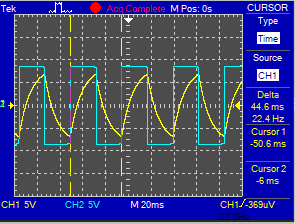
\includegraphics[width=\linewidth, height=\simheight]{images/Square-Wave-Generator-T-Cursor.png}
    \caption{$T$ from waveform for astable multivibrator as square wave generator}
    \label{fig:T from waveform for astable multivibrator as square wave generator}
\end{figure}

\subsection{Comments}
The primary characteristic to analyze is the frequency of the square wave generated by the astable multivibrator. This frequency is determined by the values of the resistors and capacitors in the timing network, as well as the characteristics of the op-amp itself.
\[ \beta = \frac{R_{1}}{R_{1}+R_{2}}\]
\[ T = 2RC \times \ln{\frac{1+\beta}{1-\beta}}\]
\[ f = \frac{1}{T}\]
Thus, \( \beta = \frac{10k}{10k + 2.2k}\), \( T = 2\times 10k \times 1\micro \times \ln{\frac{1+\beta}{1-\beta}} = 46.23 ms\), and \( f = 21.63Hz\). \\
From figure \ref{fig:T from waveform for astable multivibrator as square wave generator}, $T=44.6ms$ and $22.4Hz$ which are near the theoretical values. \\

Like the Schmitt trigger, the astable multivibrator also exhibits hysteresis behavior, resulting in two distinct threshold levels for switching the output between high and low states. These threshold levels are determined by the resistor values in the feedback network and the input resistors' ratio.
\[ |V_{ref}| = \frac{R_{1}}{R_{1} + R_{2}}  \times V_{ss}\]
Thus, $|V_{ss}|=8.5$ and \(|V_{ref}|=\frac{10k}{10k+2.2k}\times8.5=6.97V\). \\
From figure \ref{fig:$V_{ref}$ from waveform for astable multivibrator as square wave generator}, $|V_{ref}|=7.3V$ which is near the theoretical value.

\newpage

\patchcmd{\thebibliography}{\section*}{\section}{}{}

\end{document}